\documentclass[12pt, a4paper, openany]{report}
\def\VersionRapport{1.0}
\usepackage[utf8]{inputenc} % un package
\usepackage[T1]{fontenc}      % un second package
\usepackage[francais]{babel}  % un troisième package
\usepackage{layout}
\usepackage[top=2.7cm, bottom=2.5cm, left=3.5cm, right=3cm]{geometry}
\usepackage{setspace}
\frenchbsetup{StandardLists=true} % à inclure si on utilise \usepackage[french]{babel}
%\usepackage{enumitem}
\usepackage[shortlabels]{enumitem}
\usepackage{amssymb}
\usepackage{color}
\usepackage{listings}
\definecolor{dkgreen}{rgb}{0,0.6,0}
\definecolor{gray}{rgb}{0.5,0.5,0.5}
\definecolor{mauve}{rgb}{0.58,0,0.82}
\definecolor{rougecerise}{rgb}{0.73,0.043,0.043}
\lstset{frame=tb,
  %language=Matlab,
  language=JAVA,
  aboveskip=3mm,
  belowskip=3mm,
  showstringspaces=false,
  columns=flexible,
  basicstyle={\small\ttfamily},
  keywordstyle=\color{blue},
  commentstyle=\color{dkgreen},
  stringstyle=\color{mauve},
  breaklines=true,
  breakatwhitespace=true,
  tabsize=3,
  breaklines=true,
  morekeywords={matlab2tikz},
  morekeywords=[2]{1}, 
  keywordstyle=[2]{\color{black}},
  identifierstyle=\color{black},
  numbers=left,
  numberstyle={\tiny \color{black}},
  numbersep=9pt, 
  emph=[1]{for,end,break},
  emphstyle=[1]\color{red}
}
\usepackage{multirow} % pour les tableaux
\usepackage[table]{xcolor} % pour les tableaux
\usepackage{verbatim}
%\usepackage{subcaption}
\usepackage{graphicx}
\usepackage{moreverb}
\usepackage{url}
\usepackage{pst-all}
\usepackage{eso-pic,graphicx}
\usepackage{caption} 
\usepackage[colorlinks=true,urlcolor=blue,linkcolor=red]{hyperref}
\usepackage{array}
\usepackage[toc,page]{appendix}
\usepackage[off]{auto-pst-pdf}
\usepackage{hyperref} % pour le sommaire table des matières
\AddThinSpaceBeforeFootnotes % à insérer si on utilise \usepackage[french]{babel}
\FrenchFootnotes % à insérer si on utilise \usepackage[french]{babel}
\usepackage{fancyhdr}
\pagestyle{headings}
\usepackage{pifont}  %pour les puces
\usepackage{amsmath,amsfonts,amssymb} %pour les puces
\usepackage{subfig}
\usepackage{verbatim} % pour le code en annexe 
%%%%%%%colones 
\newcolumntype{R}[1]{>{\raggedleft\arraybackslash }b{#1}}
\newcolumntype{L}[1]{>{\raggedright\arraybackslash }b{#1}}
\newcolumntype{C}[1]{>{\centering\arraybackslash }b{#1}}
%%%%%%% 
\renewcommand{\appendixpagename}{Annexes}
\renewcommand{\appendixtocname}{Annexes}
\title{Theme: Compte Rendu Outils pour la Commande des Systèmes Parallèles}
\author{NAIMI \bsc{Nabil} \\ KHERBICHE \bsc{Ali}}
\date{2018-2019}
%new
\newcommand{\HRule}{\rule{\linewidth}{0.5mm}}

\begin{document}

%\selectlanguage{francais}
\pagenumbering{arabic} 
\makeatletter
\begin{titlepage}
\begin{sffamily}
\begin{center}
    % Upper part of the page. The '~' is needed because \\
    % only works if a paragraph has started.
    
\includegraphics[scale=0.5]{Logo_UT3.jpg}~\\[1cm]
    \textsc{\LARGE M1 ISTR-RODECO  }\\[1cm]
    \textsc{\Large Compte Rendu Outils pour la Commande des Systèmes Parallèles}\\[1cm]
    % Title
    \HRule \\[0.4cm] % sous de ligne
    { \huge  \textsc {Gestion de Wagonnets\\[0.4cm] }}
	\HRule \\[0.4cm] % sous de ligne
	{ \huge  \textsc {Mise en Oeuvre d'un Moniteur pour le Problème des Philosophes \\[0.4cm] }}
    \HRule \\[1cm]   % sous de ligne 
    
\includegraphics[scale=0.1]{logomaster.jpg}
    \\[1cm]
    % Author and supervisor
    \begin{minipage}{0.4\textwidth}
      \begin{flushleft} \large
         \textsc{\emph {Fait par:} \\KHERBICHE Ali\\ NAIMI Nabil}  
          \newline
          Promotion 2018-2019 \\
      \end{flushleft}
    \end{minipage}
    \begin{minipage}{0.4\textwidth}
      \begin{flushright} \large
        %%\emph{Tuteur et}
        \emph{Tuteur:\\} \textsc{M Hamid DEMMOU}
      \end{flushright}
    \end{minipage}
    \vfill
    % Bottom of the page
    {\large Avril 2018}
  \end{center}
  \end{sffamily}                
  \end{titlepage}  
\makeatother
   
%*********************** somaire **************
\renewcommand{\contentsname}{Sommaire}
\tableofcontents
%*********************** listes des figures **************
\listoffigures
%*********************** listes des tableaux **************
%\listoftables

    \begin{titlepage}
    \centering
    \vspace*{\fill}

    \vspace*{0.5cm}
    \huge\bfseries
    \textsc{Gestion de Wagonnets:\\ Spécification par Réseaux de Petri\\
    Mise en oeuvre Programmée sur PC en Langage Evolué}
    \vspace*{0.5cm}
    
    \vspace*{\fill}
    \end{titlepage}
\chapter*{\textsc{Introduction}}
\addcontentsline{toc}{chapter}{\textsc{Introduction}}

	\paragraph{} L'objet de cette manipulation est de commander un système de transfert de matières premières en vrac (sable, gravier, ...) par wagonnets entre deux postes de chargement/déchargement.
	\par Les deux points essentiels illustrés par cette manipulation sont :
	
		\begin{itemize} [label=\ding{70},font=\small \color{black}]
   		\item La spécification de la commande par réseau de Petri.
   		\item Une mise en œuvre programmée de cette spécification, sur un PC en langage évolué.
  		\end{itemize}


\par Pour chaque partie de la manipulation, on modélise le système de commande par réseau de Petri et on met en œuvre cette modélisation sur PC, en utilisant le langage C et une programmation multithreads. Pour cela il faut découper le réseau de Petri en plusieurs tâches et identifier les points
de synchronisation et/ou de communication.

\par La disposition des voies empruntées par les wagonnets et la position des postes de chargement/déchargement sont données par la figure ci-dessous.

	\begin{center}
	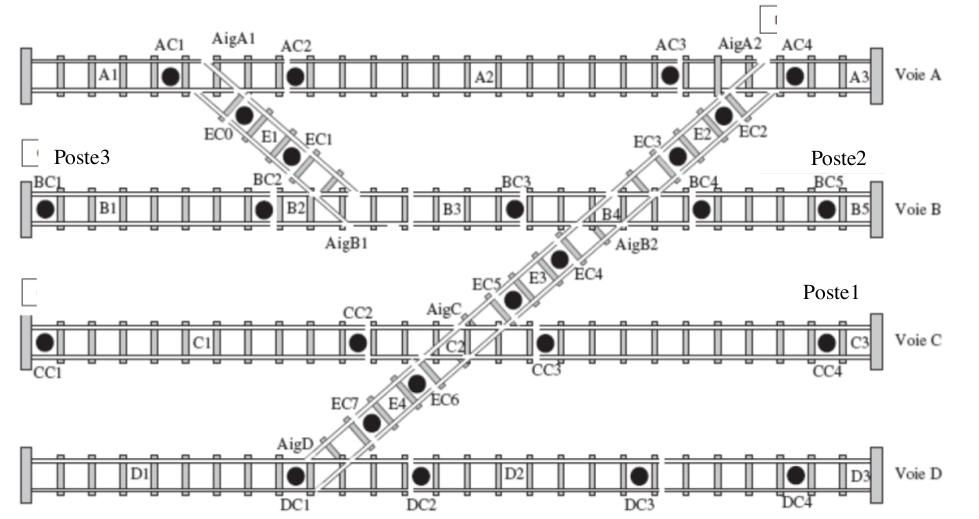
\includegraphics[scale=0.4]{maquette.png}
	\captionof{figure}{\textit{Schéma de la maquette trains. \\}}
	\label{fig4} 
	\end{center}  





\chapter{\textsc{ Modélisation du fonctionnement d'un seul wagonnet $w1$ }}
\section{\textsc{Le réseau de Petri}}
	
	\begin{center}
	%\includegraphics[scale=0.5]{sim1.png}
	\captionof{figure}{\textit{Réseau de Petri du fonctionnement d'un seul wagonnet $w1$ \\}}
	\label{fig1} 
	\end{center}  

\section{\textsc{Le code C correspondant}}
	\begin{lstlisting}
		for (i=0);
		public class main 
		import package
	\end{lstlisting}

%%%%%%%%%%%%%%%%%%%%%
	
\chapter{\textsc{ Modélisation du fonctionnement de deux wagonnets $w1$ et $w2$ }}
\section{\textsc{Le réseau de Petri}}
	
	\begin{center}
	%\includegraphics[scale=0.5]{sim1.png}
	\captionof{figure}{\textit{Réseau de Petri du fonctionnement de deux wagonnets $w1$ et $w2$ \\}}
	\label{fig2} 
	\end{center}  

\section{\textsc{Le code C correspondant}}
	\begin{lstlisting}
		for (i=0);
	\end{lstlisting}


%%%%%%%%%%%%%%%%%%%%%

\chapter{\textsc{ Modélisation du fonctionnement des trois wagonnets $w1$, $w2$ et $w3$}}
\section{\textsc{Le réseau de Petri}}
	
	\begin{center}
	%\includegraphics[scale=0.5]{sim1.png}
	\captionof{figure}{\textit{Réseau de Petri du fonctionnement de deux wagonnets $w1$, $w2$ et $w3$ \\}}
	\label{fig3} 
	\end{center}  

\section{\textsc{Le code C correspondant}}
	\begin{lstlisting}
		for (i=0);
	\end{lstlisting}

%%%%%%%%%%%%%%%%%%

\chapter*{\textsc{Conclusion}}
\addcontentsline{toc}{chapter}{\textsc{Conclusion}}

	\paragraph{}
    \begin{titlepage}
    \centering
    \vspace*{\fill}

    \vspace*{0.5cm}
    \huge\bfseries
    \textsc{Programmation en Langage JAVA\\Mise en Oeuvre d'un Moniteur pour le Problème des Philosophes\\}
    \vspace*{0.5cm}
    
    \vspace*{\fill}
    \end{titlepage}
\chapter*{\textsc{Introduction}}
\addcontentsline{toc}{chapter}{\textsc{Introduction}}

	\paragraph{} Le langage JAVA inclut la possibilité de gérer l’exclusion mutuelle entre des objets ou entre les méthodes d’un objet. Plusieurs possibilités décrites en cours peuvent être utilisées pour mettre en œuvre un moniteur. La plus adaptée est celle basée sur le type d’objet « Condition » auquel sont associées les fonctions d’attente et de signal sur Condition. Le but de la manipulation est de valider les acquis du cours en créant un programme permettant de gérer l’exécution de plusieurs processus « philosophes » partageant plusieurs ressources (les baguettes...).
	


%%\chapter{\textsc{ Mise en Oeuvre d'un Moniteur pour le Problème des Philosophes }}
\chapter{\textsc{Développement d'un programme JAVA avec des Sémaphores}}
\section{\textsc{Code JAVA}}

\subsection{\textsc{Code de la classe philosophe}}
	\begin{lstlisting}
		
package philosopher;
import java.util.concurrent.Semaphore;

	public class philosopher  extends Thread {
		private Semaphore baguetteD, baguetteG;
		private int numb_ph;
	
		public philosopher (int numb,Semaphore Bag1,Semaphore Bag2 ){
			this.numb_ph=numb;
			this.baguetteD=Bag1;
			this.baguetteG=Bag2;
		}
	
	
	public void Pense(){ //he thinks
		System.out.println("Le philosophe "+this.numb_ph+" pense.");
		try{
			Thread.sleep(2000);
		}
		catch(InterruptedException excep){}
	}

	
	public void Afaim(){ //he's hungry
		System.out.println("Le philosophe "+this.numb_ph+" a faim");
		try{
			baguetteG.acquire();
			baguetteD.acquire();
		}
		catch(InterruptedException excep){}
	}
	
	
	public void Mange(){ //he eats
		System.out.println("Le philosophe "+this.numb_ph+" mange");
		try{
			Thread.sleep(1000);
			baguetteG.release();
			baguetteD.release();
		}
		catch(InterruptedException excep){}
	}
	
	
	public void run() {
		while(true) {
		Pense();
		Afaim();
		Mange();
		}
	}
}

	\end{lstlisting}


\subsection{\textsc{Code du main}}

	\begin{lstlisting}
		
package philosopher;
import java.util.concurrent.Semaphore;

public class main_Sem { 
	public static void main (String[] args) {
		// TODO Auto-generated method stub
		Semaphore baguette[]=new Semaphore[5];
		philosopher ph[]= new philosopher [5];
		for(int i=0; i<5; i++) {
			baguette[i]=new Semaphore(1);
		}
		for(int j=0; j<5; j++) {
			ph[j] = new philosopher(j,baguette[j],baguette[(j+1)%5]);
			System.out.println("Le philosophe "+j+" a rejoint la table." );
			ph[j].start();
		}
	}
}

	\end{lstlisting}


%%%%%%%%%%%%%%%

%\chapter{\textsc{Développement d'un programme JAVA avec un Moniteur}}
%\section{\textsc{Code JAVA}}
%
%\subsection{\textsc{Code de la classe philosophe}}
%
%
%
%\subsection{\textsc{Code du main}}


\chapter*{\textsc{Conclusion}}
\addcontentsline{toc}{chapter}{\textsc{Conclusion}}

	\paragraph{} Nous n'avons malheureusement pas pu finir la partie moniteur à défaut de temps. Mais la partie sémaphore est une pleine réussite pour nous car non seulement nous avons pu réussir cette partie mais aussi nous avons approfondi nos connaissance sur le langage JAVA.\\  
%\input{chap3.tex}
%\input{conclusion.tex}
%\input{annexes.tex}
%*********************** Bibliographie ************ 
\bibliographystyle{alpha}
\bibliography{biblio}  

\end{document}